\documentclass[11pt]{elegantbook}
\definecolor{structurecolor}{RGB}{40,58,129}
\linespread{1.6}
\setlength{\footskip}{20pt}
\setlength{\parindent}{0pt}
\newcommand{\argmax}{\operatornamewithlimits{argmax}}
\newcommand{\argmin}{\operatornamewithlimits{argmin}}
\elegantnewtheorem{proof}{Proof}{}{Proof}
\elegantnewtheorem{claim}{Claim}{prostyle}{Claim}
\DeclareMathOperator{\col}{col}
\title{\textbf{STAT 426}}
\author{Wenxiao Yang}
\institute{Department of Mathematics, University of Illinois at Urbana-Champaign}
\date{}
\setcounter{tocdepth}{2}
\cover{cover.jpg}
\extrainfo{All models are wrong, but some are useful.}

% modify the color in the middle of titlepage
\definecolor{customcolor}{RGB}{32,178,170}
\colorlet{coverlinecolor}{customcolor}
\usepackage{cprotect}

\addbibresource[location=local]{reference.bib} % bib

\begin{document}

\maketitle
\frontmatter
\tableofcontents
\mainmatter

\chapter{Basic of Categorical Data}
\section{Variable Measurement}
\begin{center}\begin{figure}[htbp]
    \centering
    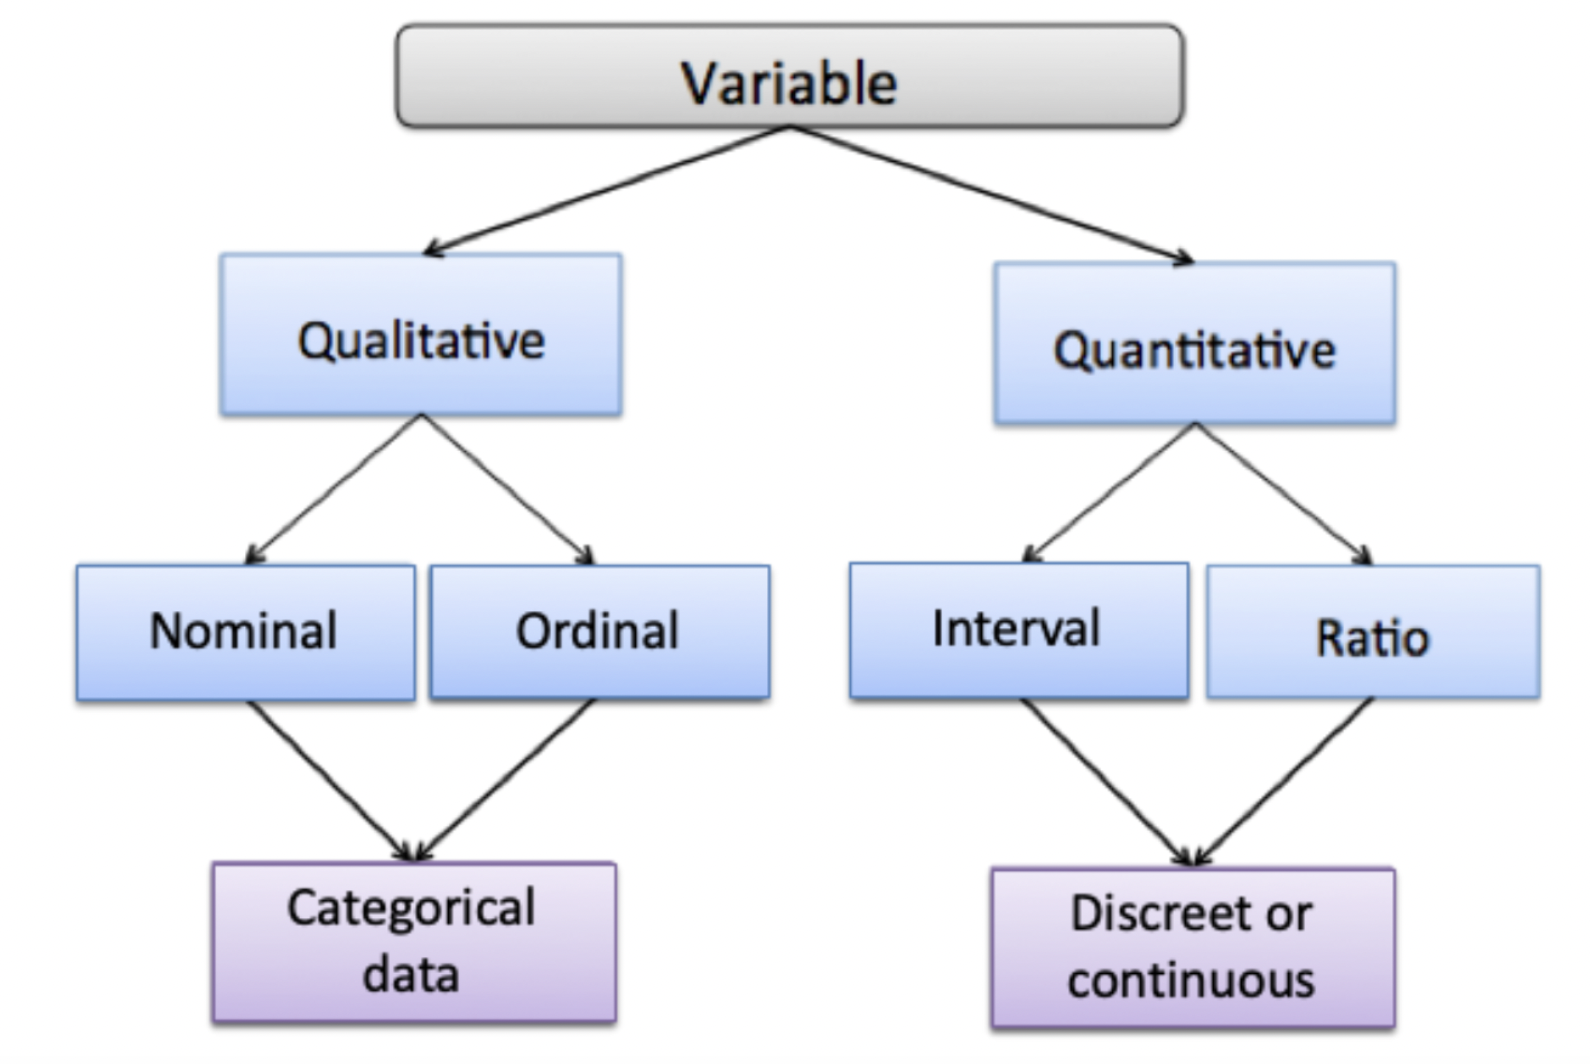
\includegraphics[scale=0.3]{p1.png}
    \caption{Variable Type}
    \label{}
\end{figure}\end{center}
\begin{enumerate}[a)]
    \item Nominal: Categories do not have a natural order. Ex. blood type, gender.
    \item Ordinal: Categories have a natural order. Ex. low/middle/high education level
    \item Interval: There is a numerical distance (difference between two different values is meaningful) between any two values.
    Ex. blood pressure level, 100 blood pressure doesn't mean the double degree of 50 pressure.
    \item Ratio: An interval variable where ratios are valid (presence of absolute zero, i.e. zero is meaningful). Ex. weight, 4g is double degree of 2g, distance run by an athlete.
\end{enumerate}
\subsection*{Levels of measurements}
A variable's level of measurement determines the statistical methods to be used for its analysis.
\begin{center}
    Variables hierarchy: Ratio $>$ Interval $>$ Ordinal $>$ Nominal
\end{center}
Statistical methods applied to variables at a lower level can be used with variables at a higher level, but the contrary is not true.

\section{Statistical Inference for Categorical Data}
There is a distribution $F(\beta)$ with p.d.f. (p.m.f.) $f(x\mid\beta)$, where $\beta$ a generic unknown parameter and $\hat{\beta}$ the parameter estimate.
\subsection{Maximum likelihood Estimation (MLE)}
Given a set of observations $\vec{x}=(x_1,...,x_n)$, the likelihood function of these observations with parameter $\beta$ is $l(\vec{x}\mid\beta)$. We want to find parameter $\hat{\beta}$ that maximizes the likelihood function,$$\hat{\beta}=\arg\max_{\beta} l(\vec{x}\mid\beta)$$
which is also equivalent to maximizing the logarithm of the likelihood function $L(\vec{x}\mid\beta) = \log(l(\vec{x}\mid\beta))$, $$\hat{\beta}=\arg\max_{\beta}L(\vec{x}\mid\beta)$$

\begin{definition}[score function]
    The score function is $$u(\beta,\vec{x})=\frac{\partial L(\vec{x}\mid \beta)}{\partial \beta}=\frac{\nabla_{\beta} l(\vec{x}\mid \beta)}{l(\vec{x}\mid \beta)}$$
\end{definition}
\begin{lemma}[mean of score function]
    The mean of score function is $0$,
    $$\mathbb{E}_{\vec{x}}u(\beta,\vec{x})=0$$
\end{lemma}
\begin{proof}
    \begin{equation}
        \begin{aligned}
            \mathbb{E}_{\vec{x}}u(\beta,\vec{x})&=\int_{\vec{x}}l(\vec{x}\mid \beta)\frac{\nabla_{\beta} l(\vec{x}\mid \beta)}{l(\vec{x}\mid \beta)}d \vec{x}\\
            &=\int_{\vec{x}}\nabla_{\beta} l(\vec{x}\mid \beta)d \vec{x}\\
            &=\nabla_{\beta}\left(\int_{\vec{x}}l(\vec{x}\mid \beta)d \vec{x}\right)\\
            &=\nabla_{\beta}1=0
        \end{aligned}
        \nonumber
    \end{equation}
\end{proof}

\begin{lemma}[variance of score function]
    The variance of the score function is $$\textnormal{Var}_{\vec{x}}(u(\beta, \vec{x}))= \mathbb{E}_{\vec{x}}\left(u(\beta, \vec{x})u(\beta, \vec{x})^T\right)$$
\end{lemma}
\begin{proof}
    Prove by the zero mean.
\end{proof}

\begin{definition}[Fisher information]
    The (Fisher) information is $$\iota(\beta)=-\mathbb{E}_{\vec{x}}\left(\frac{\partial^2 L(\vec{x}\mid\beta)}{\partial \beta^2}\right)$$
\end{definition}
\begin{lemma}
    The Fisher information is equal to the variance of score function.
    $$\textnormal{Var}_{\vec{x}}(u(\beta, \vec{x}))=\mathbb{E}_{\vec{x}}\left(u(\beta,\vec{x})u(\beta,\vec{x})^T\right)=-\mathbb{E}_{\vec{x}}\left(\frac{\partial^2 L(\vec{x}\mid\beta)}{\partial \beta^2}\right)=\iota(\beta)$$
\end{lemma}
\begin{proof}
    \begin{equation}
        \begin{aligned}
            \mathbb{E}_{\vec{x}}\left(\frac{\partial^2 L(\vec{x}\mid\beta)}{\partial \beta^2}\right)=\mathbb{E}_{\vec{x}}\frac{\partial \frac{\nabla_{\beta} l(\vec{x}\mid \beta)}{l(\vec{x}\mid \beta)}}{\partial \beta}
        \end{aligned}
        \nonumber
    \end{equation}
\end{proof}

\begin{proposition}
    When the sample $x$ is made up of i.i.d. observations, the covariance matrix of the maximum likelihood estimator $\hat{\beta}$ is approximately equal to the inverse of the information matrix. $$\textnormal{Cov}(\hat{\beta})\approx(\iota(\beta))^{-1}$$
\end{proposition}
\begin{proof}
    Use $\vec{x}=x_1,...,x_n$ denote the $n$ i.i.d. observations. The log-likelihood of the sample is $$L(\beta,\vec{x})=\sum_{i=1}^n\log(l(\beta,x_i))$$
\end{proof}















\end{document}